\chapter{Analiza nawiązanej komunikacji}
    \begin{figure}[h!]
    \centering
    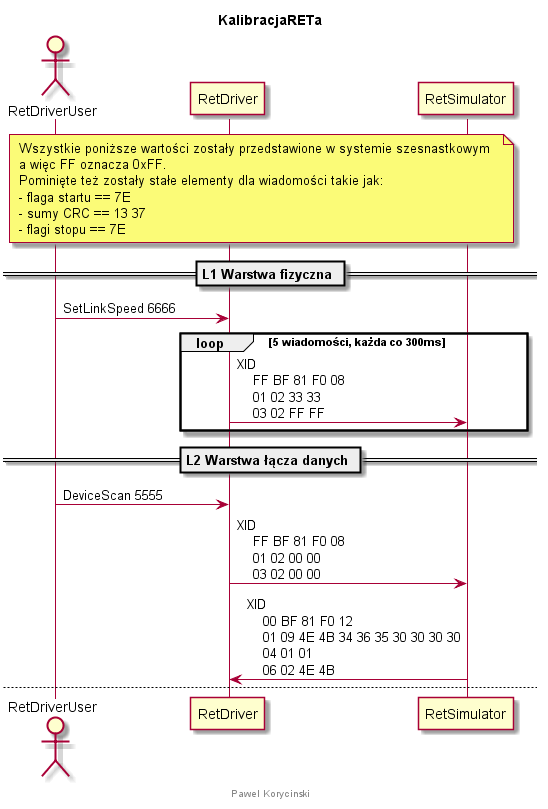
\includegraphics[scale=0.70]{out/Diagramy/UML_DiagramOfSequence_New/KalibracjaRETa-page1.png}
    \caption{Ustanowienie prędkości połączenia wraz z początkowym skanowaniem urządzeń}
    \end{figure}
    \newpage

    Na diagramach sekwencji przedstawiono komendy wywoływane przez użytkownika
    symulatora wraz z zawartościami ramek pochodzących z urządzenia nadrzędnego oraz
    wartościami ramek przychodzących z urządzenia podrzędnego.
    W celu analizy procesu komunikacji, w opisie skupiono sie na cechach charakterystycznych
    dla poszczególnej ramki czy komendy, o których nie wspomniano we wcześniejszych rozdziałach.
    
    \section{Ustanowienie prędkości połączenia}
    Parametrem tej komendy jest adres portu 6666, z którego korzysta sterownik
    do nawiązania połączenia typu tcp na adresie 127.0.0.1 wraz z symulatorem urządzenia
    przy zastosowaniu wzorca Publish-Subscribe. Podczas tego połączenia protokół AISG 2.0 
    nie zakłada oczekiwania na odpowiedź od urządzenia podrzędnego oraz użyta biblioteka
    ZeroMQ również nie udostępnia możliwości wysłania odpowiedzi na taką wiadomość.

    \section{Skanowanie urządzeń}
    Parametrem tej komendy jest adres portu 5555, z którego korzysta sterownik
    do nawiązania połączenia typu tcp na adresie 127.0.0.1 wraz z symulatorem urządzenia,
    przy zastosowaniu wzorca Żadanie-Odpowiedź. Jest to wzorzec, który zakłada otrzymanie 
    odpowiedzi na każdą wysłaną wiadomość, zanim kolejna zostanie nadana. Opisany mechanizm komunikacji
    aplikowalny jest również do wszystkich poniższych komend.
    Ciekawym elementem tej wiadomości jest to, że otrzymano kod producenta zarówno
    w osobnym parametrze jak i jako składową unikalnego identyfikatora urządzenia.

    \section{Żadanie adresacji}
    Tutaj po raz pierwszy można zaobserwować zmienioną wartość pola adresu dla wiadomości
    przychodzącej. Oznacza to, że urządzenie podrzędne zaakceptowało żadanie adresacji 
    oraz identyfikuje się w trakcie rozmowy z urządzeniem nadrzędnym pod adresem 0x03 co
    jest prawdą dla każdej następnej wiadomości.
 
    \begin{figure}[h!]
    \centering
    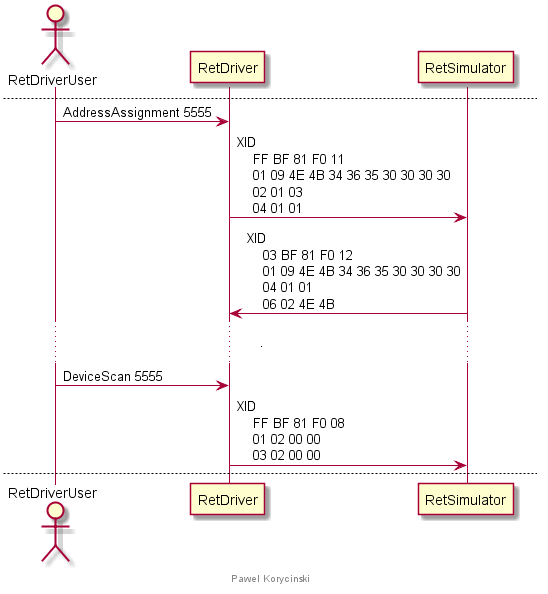
\includegraphics[scale=0.75]{out/Diagramy/UML_DiagramOfSequence_New/KalibracjaRETa-page2.png}
    \caption{Żadanie adresacji oraz dodatkowe skanowanie urządzeń}
    \end{figure}

    \section{Ponowne skanowanie urządzeń}
    W zakresie tego projektu komunikacja nawiązywana jest z jednym urządzeniem, a więc dlaczego
    ponownie wysłano wiadomość skanowania ? Otóż na tę wiadomość urządzenie nadrzędne
    nie powinno otrzymać odpowiedzi, gdyż jedynie urządzenia niezaadresowane mogą na nie 
    odpowiedzieć, co jest podstawową metodą dodatkowej weryfikacji powodzenia procedury
    adresowania.

    \section{Negocjacje parametrów HDLC}
    Cechą negocjacji parametrów przy pomocy ramek XID jest to, że jeśli żądana wartość jest wspierana przez
    urządzenie podrzędne, to odpowie ono wiadomością zawierającą te same parametry oraz te same wartości. 
    W przeciwnym wypadku otrzymanymi wartościami parametrów będą największe możliwe przez nie wspierane.
    Zaobserwowano to zjawisko w przypadku negocjacji wielkości payloadu dla wysłanej oraz otrzymanej ramki informacyjnej.
    Urządzenie nadrzędne próbowało ustanowić dopuszczalną liczbę bitów na \{0xF0, 0x2D, 0x00, 0x00\} co daje wartość 61485,
    lecz urządzenie podrzędne odpowiedziało \{0x50, 0x02, 0x00, 0x00\} co po konwersji na system dziesiętny daje 20482 bity.

    \section{Przejście na normalny tryb komunikacji}
    Jako odpowiedź na tę wiadomość urządzenie otrzyma ramkę, która zawiera wartość 0x73, co oznacza że 
    potwierdza ono żądane oczekiwanie.

    \section{Kalibracja}
    W związku z tym, że oczekiwanie kalibracji przesłano przy pomocy ramki informacyjnej, bajt kontrolny posiada
    charakterystyczną metodę jego ewaluacji przedstawioną wcześniej. Diagram sekwencji
    potwierdza to, gdyż wiadomość odebrana przez urządzenie nadrzędne posiada wartość równą 0x30.
    Ramka odebrana, na wyznaczenie liczby bajtów budujących odpowiedź posiada zarezerowane dwa bajty. 
    Ciekawą obserwacją jest to, że odpowiedź równą 0x00 czyli OK można by zapisać przy pomocy jedynie jednego bajta, lecz optymalizacja
    pamięci nie jest tutaj zastosowana.

    \begin{figure}[h!]
    \centering
    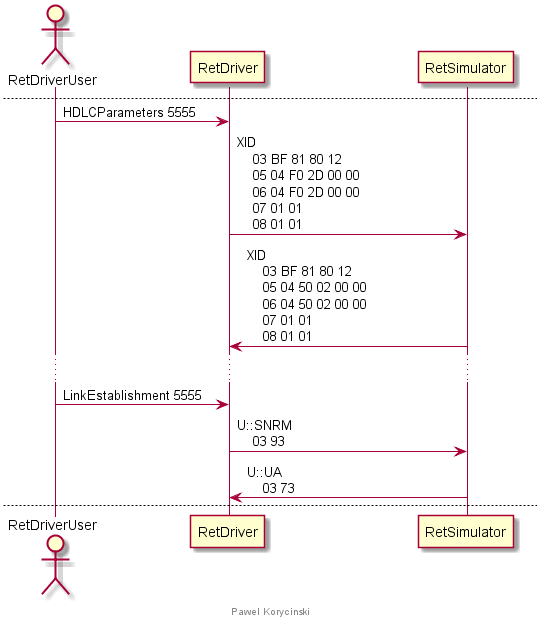
\includegraphics[scale=0.75]{out/Diagramy/UML_DiagramOfSequence_New/KalibracjaRETa-page3.png}
    \caption{Negocjacja rozmiaru okna oraz payloadu ramki informacyjnej oraz ustanowienie normalnego trybu komunikacji}
    \end{figure}

    \begin{figure}[h!]
    \centering
    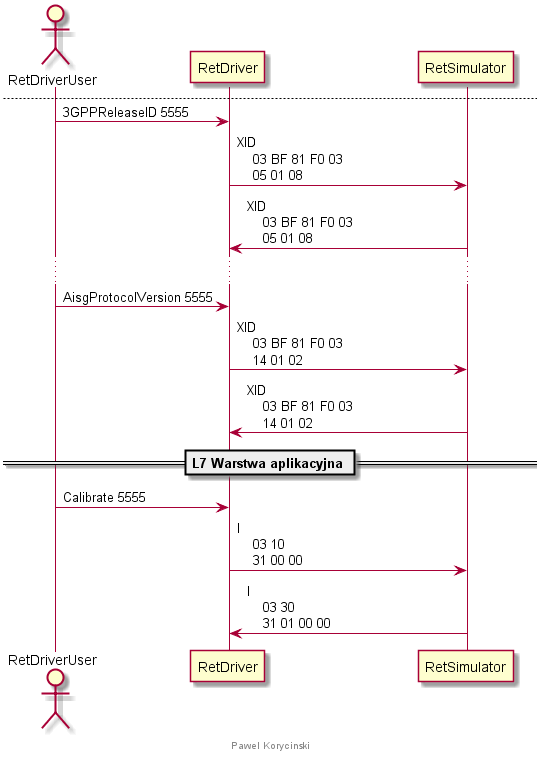
\includegraphics[scale=0.75]{out/Diagramy/UML_DiagramOfSequence_New/KalibracjaRETa-page4.png}
    \caption{Negocjacja pozostałych parametrów HDLC oraz żadanie kalibracji urządzenia}
    \end{figure}

